%% Preamble
\documentclass[usenames,dvipsnames,tikz]{article}

%% Dependencies
\usepackage{xeCJK}
\usepackage[T1]{fontenc}
\usepackage[utf8]{inputenc}
\usepackage{amsmath}
\usepackage{color}
\usepackage{xcolor}
\usepackage[b4paper,landscape,nohead,margin=2cm]{geometry}
\usepackage{tikz}
\usepackage{tikz-cd}
\usepackage{amsfonts}
\usetikzlibrary{shapes,mindmap,shadows,backgrounds}
\usetikzlibrary{cd,matrix}

%% Settings
\definecolor{shallowyellow}{RGB}{245,245,204}
\def\anno#1#2#3{\node[anno,#3] at (#2) {\textbf{\large #1}}}
\def\annop#1#2{\node[anno,xshift=-5cm] at (#2) {\textbf{\large #1}}}

%% Stylish
\pagestyle{empty}
\pagecolor{shallowyellow}
\tikzstyle{root}+=[font=\Huge]
\tikzstyle{node}+=[concept color=teal]
\tikzstyle{cons}+=[concept color=purple]
\tikzstyle{chain}+=[concept color=darkgray]
\tikzstyle{anno}=[annotation,everynode,above,fill=black!50,text width=8cm,inner sep=4mm]
\tikzstyle{group}+=[mindmap,grow cyclic,concept color=darkgray,every node/.append style={everynode,concept}]
\tikzstyle{catethe}=[inner sep=12mm,row sep=2em,column sep=3em]
\tikzstyle{catebg}=[scale=2,fill=black!15,rounded corners=4mm]
\tikzstyle{everynode}+=[text=white,scale=1.2,circular drop shadow]
\tikzstyle{level 1 concept}+=[level distance=5.2cm,font=\huge]
\tikzstyle{level 2 concept}+=[level distance=3.8cm,font=\Large]


%% Document
\begin{document}

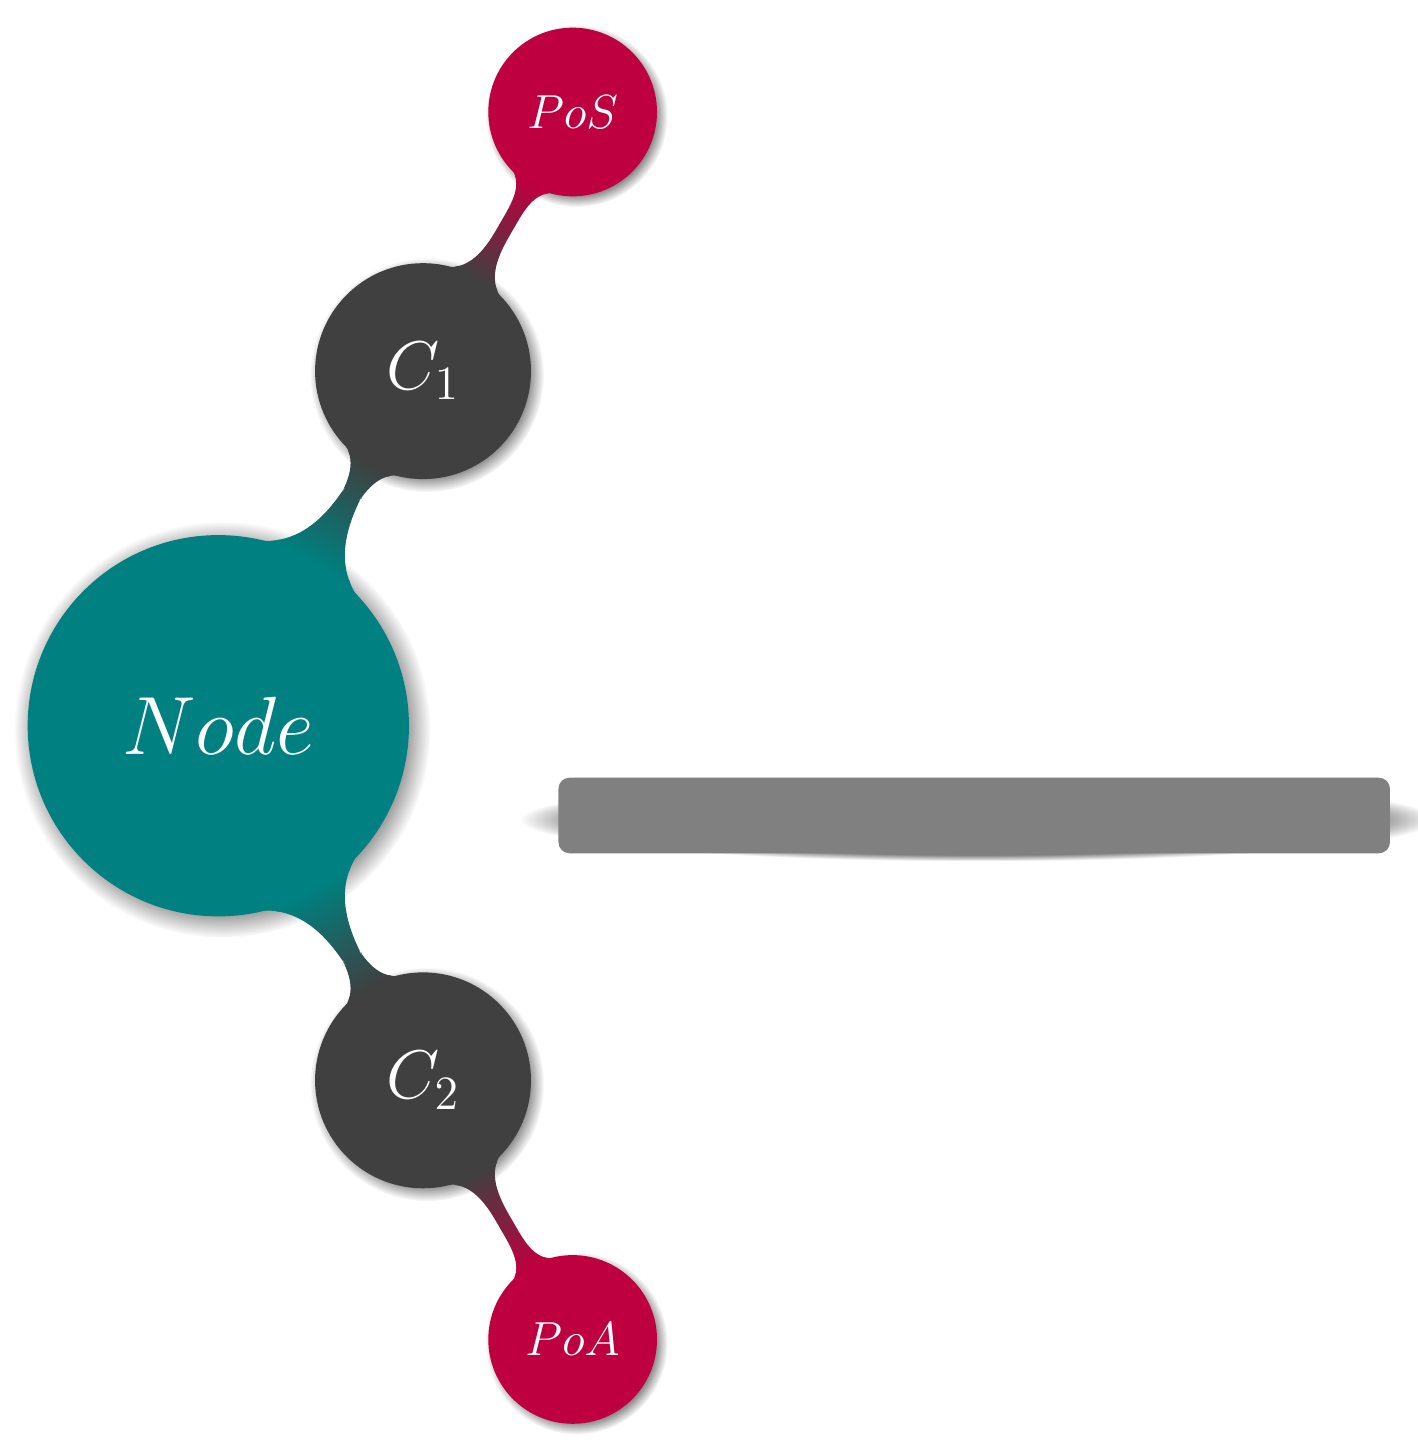
\begin{tikzpicture}
  \path[group,node,level 1/.append style={sibling angle=120}]
  node[root] (node) {$Node$}
  child[chain] {node {$C_2$} child[cons] {node {$PoA$}}}
  child[chain] {node {$C_1$} child[cons] {node {$PoS$}}};
  \anno{}{node.east}{xshift=6cm,yshift=-1.5cm};
\end{tikzpicture}


%  放弃去从原有区块链中拓展、定制新的区块链,而是假设应用程序会分离在各种不同的链上
%  代理验证与合并工作量
%  Plasma + Binary star(Union Plasma),可以想象一个节点的守护进程为该节点所参与的区块链的子链的一个节点


\end{document}